\documentclass[11pt]{article}

\usepackage[margin=1in]{geometry}
\usepackage{amsmath,amssymb,amsthm}
\usepackage{physics}
\usepackage{siunitx}
\usepackage{enumitem}
\usepackage{graphicx}
\usepackage{hyperref}
\usepackage{pdfpages}

\title{The Solar System HW3}
\author{Mediumunwell}
\date{\today}

\begin{document}
\maketitle

\section*{Problem 1}
Go over your midterm and the midterm solutions so that you understand how to ace these
problems if you ever see them again. Bring questions to class.

\subsection*{Solution}
Completed by review of midterm and posted solutions. Specific questions will be brought to class.

\section*{Problem 2}
For this question, you will use the Solar System Collisions website at
\url{http://janus.astro.umd.edu/astro/impact/}.
\begin{enumerate}[label=(\alph*)]
\item Investigate collisions with the planets Mars, Venus, and Earth. Determine the maximum-sized
rocky object that is destroyed in the planet's atmosphere to two significant figures.
Use the default collision speed of $\SI{20}{km/s}$.
\item How much energy is released by the largest airbursts on each planet (in Megatons)?
How often does this happen?
\item What are the smallest craters that can be produced on these planets?
\item Saturn's satellite Titan has an atmosphere about ten times thicker than Earth's.
What sorts of impact craters might you expect to find on its surface?
\end{enumerate}

\subsection*{Solution}
This problem requires interactive outputs from the collision simulator.
Populate the measured values below after running the website.

\begin{center}
\begin{tabular}{lccc}
\hline
Quantity & Mars & Venus & Earth \\
\hline
Largest fully destroyed rocky object & \_\_ & \_\_ & \_\_ \\
Largest-airburst energy (Mt) & \_\_ & \_\_ & \_\_ \\
Event frequency & \_\_ & \_\_ & \_\_ \\
Smallest crater size & \_\_ & \_\_ & \_\_ \\
\hline
\end{tabular}
\end{center}

For part (d), expected qualitative conclusion: a much thicker atmosphere filters out smaller and
moderate impactors more effectively, so Titan should show fewer small craters and a crater
population biased toward larger, higher-energy impacts that can survive atmospheric deceleration
and ablation.

\section*{Problem 3}
Pressure at Earth's center.
\begin{enumerate}[label=(\alph*)]
\item Find the accepted value from Appendix E. Compare with the predictions of a uniform
density planet by first deriving and then applying Eq. 3.21. Finally, work out the fraction
of the pressure that comes from the core, the part of the planet with $r < R/2$.
\item Make a more realistic approximation by considering a two-component Earth with an iron core
mass $m_c = 1.98 \times 10^{24}\,\si{kg}$ and radius $r_c = \SI{3485}{km}$ and a mantle
mass $m_m = 4.00 \times 10^{24}\,\si{kg}$ and radius $r_m = \SI{6371}{km}$. Determine average
core and mantle densities. Use linearly increasing gravity in the core and approximately constant
gravity in the mantle. Find the gravity at the core-mantle boundary, compare with surface gravity,
then compute and sum the core and mantle contributions to central pressure.
\end{enumerate}

\subsection*{Solution}
Use hydrostatic equilibrium:
\[
\frac{dP}{dr} = -\rho g(r)
\]

For a uniform-density sphere, $M(r)=\frac{4\pi}{3}\rho r^3$, so
\[
g(r)=\frac{GM(r)}{r^2}=\frac{4\pi G\rho}{3}r
\]
therefore
\[
\frac{dP}{dr}=-\frac{4\pi G\rho^2}{3}r
\]
with $P(R)=0$ gives
\[
P(r)=\frac{2\pi G\rho^2}{3}(R^2-r^2)
\]
and central pressure
\[
P_c=\frac{2\pi G\rho^2R^2}{3}=\frac{3GM^2}{8\pi R^4}
\]

Using Earth's mean density $\rho\approx\SI{5514}{kg/m^3}$ and
$R=\SI{6.371e6}{m}$:
\[
P_{c,\mathrm{uniform}} \approx \SI{1.73e11}{Pa}=\SI{173}{GPa}
\]

Accepted value (Appendix E):
\[
P_{c,\mathrm{accepted}} \approx \SI{3.6e11}{Pa}=\SI{360}{GPa}
\]
So the uniform model underestimates by about a factor of $\sim 2.1$.

For the fraction from $r<R/2$ in the uniform model:
\[
\frac{\int_0^{R/2} \rho g\,dr}{\int_0^R \rho g\,dr}
=\frac{\int_0^{R/2} r\,dr}{\int_0^R r\,dr}
=\frac{(R/2)^2}{R^2}=\frac{1}{4}
\]
So $25\%$ of $P_c$ comes from $r<R/2$ and $75\%$ from $R/2<r<R$.

Now the two-component model:
\[
\rho_c = \frac{m_c}{\frac{4\pi}{3}r_c^3}
\approx \SI{1.12e4}{kg/m^3}
\]
\[
\rho_m = \frac{m_m}{\frac{4\pi}{3}(r_m^3-r_c^3)}
\approx \SI{4.42e3}{kg/m^3}
\]

Core-mantle boundary gravity:
\[
g_{\mathrm{cmb}}=\frac{Gm_c}{r_c^2}\approx \SI{10.88}{m/s^2}
\]
Surface gravity from the same masses:
\[
g_s=\frac{G(m_c+m_m)}{r_m^2}\approx \SI{9.83}{m/s^2}
\]
These are close, so using approximately constant mantle gravity is reasonable.

Core contribution (linear $g$ in core):
\[
P_{c,\mathrm{core}}=\int_0^{r_c}\rho_c\frac{Gm_c}{r_c^3}r\,dr
=\frac{\rho_cGm_c}{2r_c}
\approx \SI{2.12e11}{Pa}=\SI{212}{GPa}
\]

Mantle contribution with
$g_{\mathrm{avg}}=(g_{\mathrm{cmb}}+g_s)/2\approx \SI{10.36}{m/s^2}$:
\[
P_{c,\mathrm{mantle}}\approx \rho_m g_{\mathrm{avg}}(r_m-r_c)
\approx \SI{1.32e11}{Pa}=\SI{132}{GPa}
\]

Total:
\[
P_{c,\mathrm{two\mbox{-}layer}}\approx P_{c,\mathrm{core}}+P_{c,\mathrm{mantle}}
\approx \SI{3.44e11}{Pa}=\SI{344}{GPa}
\]
This is much closer to the accepted $\sim\SI{360}{GPa}$ than the uniform-density value.

\section*{Problem 4}
Impact pressure.
\begin{enumerate}[label=(\alph*)]
\item The pressure produced by an impact depends on speed $v$, impactor radius $R$, and density
$\rho$. Use dimensional analysis for
\[
P=C\rho^xR^yv^z
\]
\item Determine $C$ using momentum flux arguments for a normally incident impact.
\item Evaluate $P$ for $R=\SI{10}{km}$, $\rho=\SI{3}{g/cm^3}$,
$v=\SI{20}{km/s}$ and compare with Earth's central pressure.
\end{enumerate}

\subsection*{Solution}
Dimensions:
\[
[P]=M L^{-1}T^{-2},\quad [\rho]=ML^{-3},\quad [R]=L,\quad [v]=LT^{-1}
\]
So
\[
ML^{-1}T^{-2}=(ML^{-3})^xL^y(LT^{-1})^z
=M^xL^{-3x+y+z}T^{-z}
\]
Match exponents:
\[
x=1,\quad z=2,\quad -3x+y+z=-1\Rightarrow y=0
\]
hence
\[
P=C\rho v^2
\]

For $d\ll R$, in time $dt$ the impactor sweeps target mass
\[
dm=\rho A\,v\,dt
\]
with frontal area $A=\pi r^2$.
Accelerating that mass from $0$ to $v$ gives
\[
d p = v\,dm \Rightarrow
F=\frac{dp}{dt}=\rho A v^2
\]
Therefore
\[
P=\frac{F}{A}=\rho v^2
\]
so
\[
C=1
\]

Numerical value:
\[
\rho=\SI{3}{g/cm^3}=\SI{3000}{kg/m^3},\quad v=\SI{2.0e4}{m/s}
\]
\[
P=\rho v^2=3000(2.0\times10^4)^2
=\SI{1.2e12}{Pa}=\SI{1200}{GPa}
\]
Compared with Earth's center pressure $\sim\SI{360}{GPa}$:
\[
\frac{P_{\mathrm{impact}}}{P_{c,\oplus}}\approx\frac{1200}{360}\approx3.3
\]
Thus impact-generated pressures can exceed deep-interior pressures, consistent with formation
of high-pressure mineral phases and shock metamorphism near large impact sites.

\section*{Problem 5}
Do the optional online mid-semester class evaluation for extra credit points.

\subsection*{Status}
Pending optional submission.

\section*{Reference Assignment PDF}
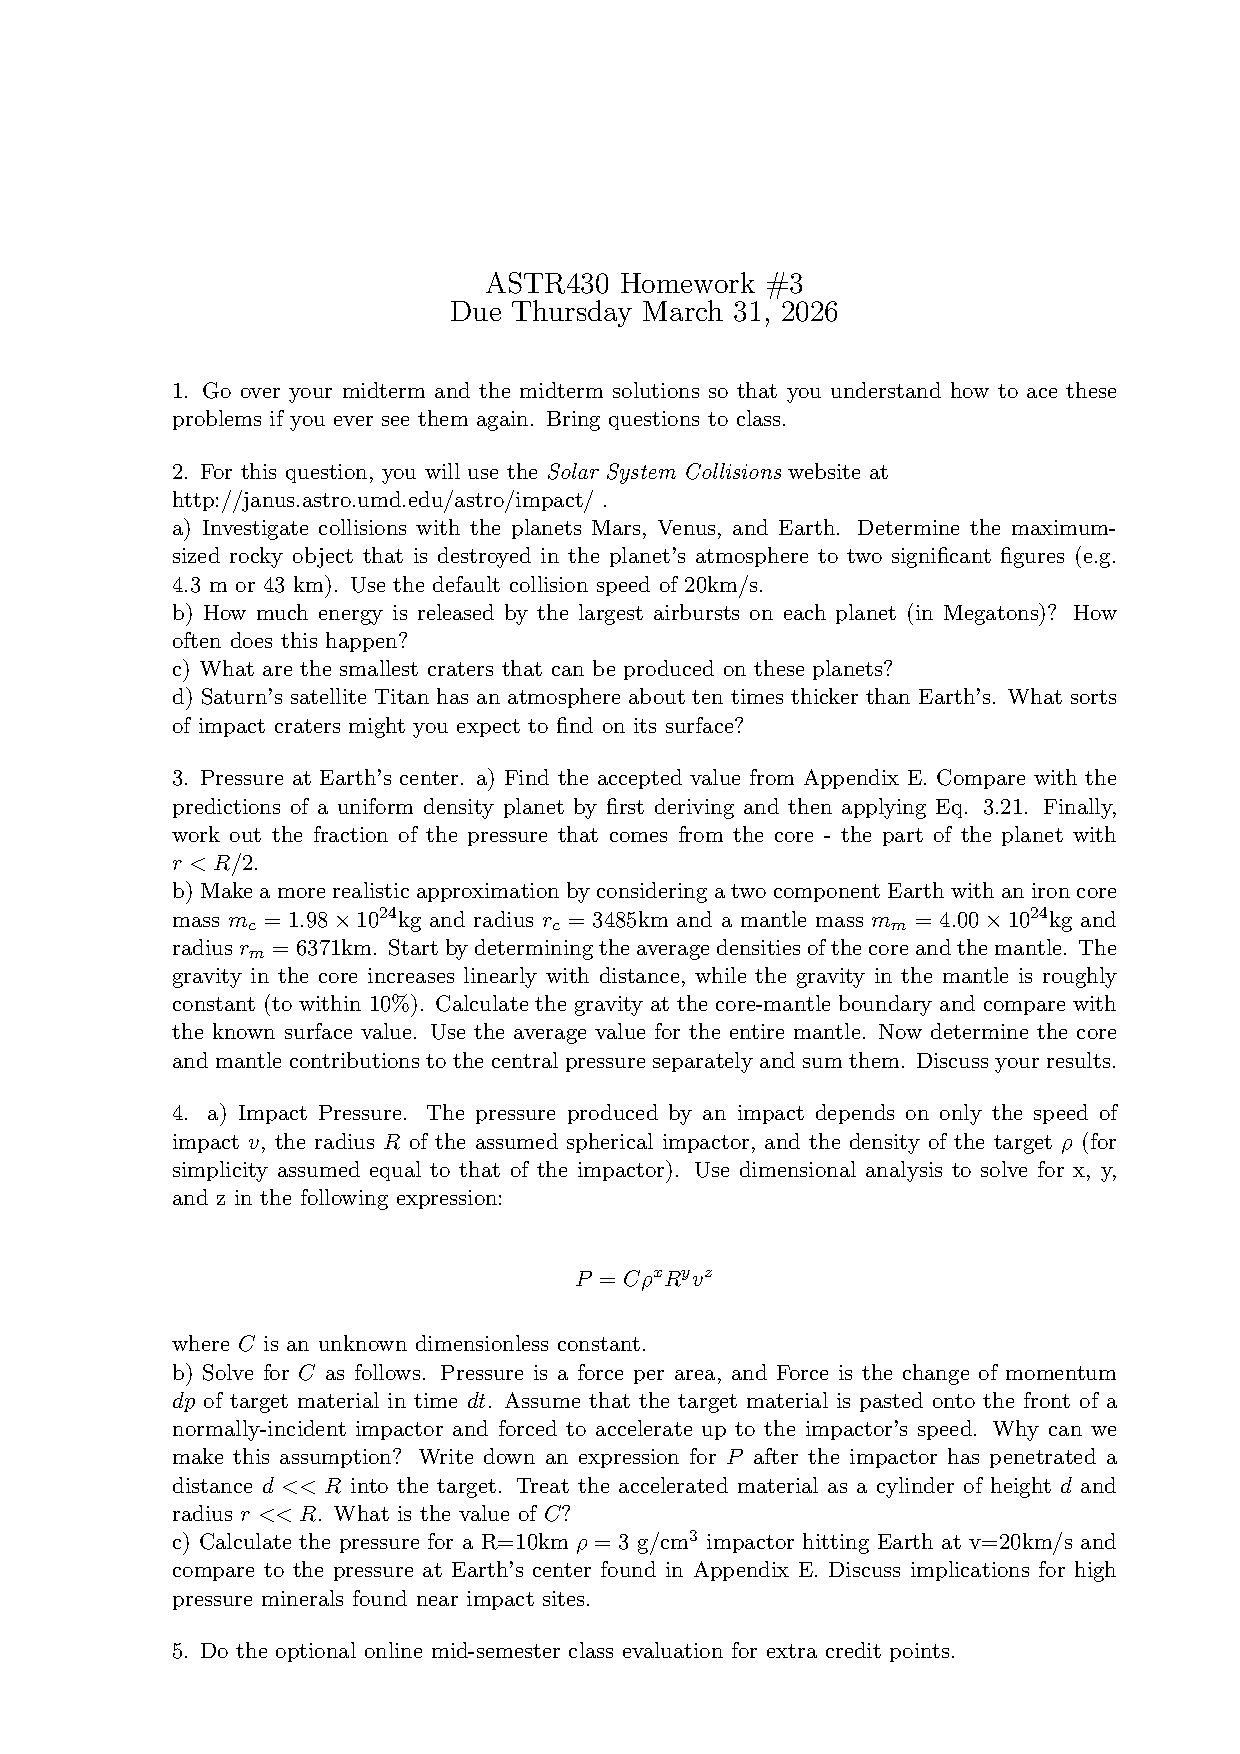
\includepdf[pages=-]{hw3.pdf}

\end{document}